\section{System Implementation}

  In this section, we describe the implementation of Lever. We have implemented Lever based on a popular open-source distributed, batch stream processing system called Spark Streaming \cite{spark-streaming}, which is an extension of cluster computing framework Apache Spark \cite{spark}. We choose Spark Streaming because it is a typical batch stream processing system based on Spark, a fast and general engine for large-scale data processing which powers a stack of libraries including SQL, machine learning, graph processing and stream processing. Spark Streaming has been widely adopted by academic community and industrial community, and also been deployed on production clusters of hundreds of thousands of corporations. In this section, we describe the details of our system implementation. The source code of our system can be found at \url{http://spark-packages.org/package/trueyao/spark-lever}.
  \begin{figure}[htbp]
    \centering
    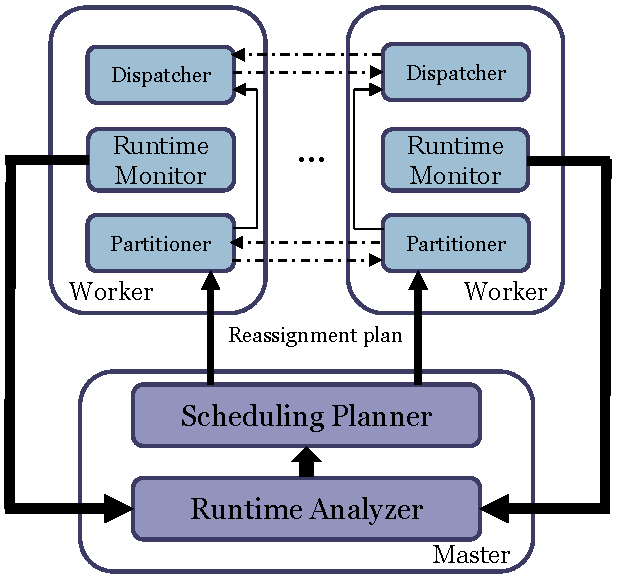
\includegraphics[width=0.35\textwidth]{Figure7}
    \caption{Implementation of Lever}
    \label{Fig. 10:}
  \end{figure}

  Figure 10 overviews the implementation of Lever. We add two components i.e. Runtime Analyzer and Scheduling Planner to master and three components i.e. Runtime Monitor, Partitioner and Dispatcher to worker, respectively. Runtime Monitor which locates in each worker periodically detects worker node information such as load and processing speed, then reports to Runtime Analyzer. By analyzing these information combined with jobs' detailed execution information, Runtime Analyzer identifies the stragglers and evaluate each node's computational capability. These results will be passed to Scheduling Planner for pre-scheduling decisions. Scheduling Planner should make a reassignment plan about how to partition and pre-schedule stragglers' work to other nodes. Partitioner is responsible for partition straggler's excess work according to specified proportion which is derived from Scheduling Planner. Dispatcher distributes every piece of partitioned work in current straggler to corresponding helpers.

  \textbf{Runtime Monitor.} \emph{Runtime Monitor} locates in each worker and periodically detects worker node information. We add some functions in \emph{executor}. When tasks are running in one executor, we can collect useful metrics such as task finish time and task's input data size through our function. We also add an accumulator in \emph{worker}. If there is one task completed, these metrics about this task is encapsulated into a message which will be sent to accumulator after this. Accumulator gathers these messages and reports to \emph{Runtime Analyzer} through an asynchronous RPC based on Akka.

  \textbf{Runtime Analyzer.} Once one batch has finished, \emph{Runtime Analyzer} begins to analyze the statistics information from \emph{Runtime Monitor}. We create a new component which maintains a table i.e. \emph{HashMap} in \emph{master}. This table is used for recording and updating workers' information. This component mainly consists of many massage receiving operations and two essential functions. One is for updating table, another is for identifying stragglers and evaluating capability.

  \textbf{Scheduling Planner.} This component receives messages from \emph{Runtime Analyzer}. It includes a main function which is responsible for running our capability-aware pre-scheduling algorithm and a output table which records pre-scheduling data assignment plan. And we also add some callback functions in \emph{JobScheduler} and \emph{TaskScheduler} in order to get scheduling information feedback and adjust task scheduling.

  \textbf{Partitioner.} We modify the \emph{BlockGenerator} and the \emph{ReceiverSupervisorImpl} to implement the Partitioner. We add a partition function \emph{splitBlockBuffer} to divide the receiving buffer into specified data share. And these fragments are delivered to \emph{BlockManager} as so called \emph{block} first(register the meta data such as block size and location to \emph{BlockManager}).

  \textbf{Dispatcher.} Function \emph{reallocateBlock} is the core of Dispatcher. This component carry out two things. One is getting the host name which data piece will be assigned to from the assignment plan. And another is invoking the \emph{blockTransferService} to transfer block. We modify the system call \emph{uploadBlockSync} in Lever to implement the remote block assignment.
